
%% bare_conf.tex
%% V1.3
%% 2007/01/11
%% by Michael Shell
%% See:
%% http://www.michaelshell.org/
%% for current contact information.
%%
%% This is a skeleton file demonstrating the use of IEEEtran.cls
%% (requires IEEEtran.cls version 1.7 or later) with an IEEE conference paper.
%%
%% Support sites:
%% http://www.michaelshell.org/tex/ieeetran/
%% http://www.ctan.org/tex-archive/macros/latex/contrib/IEEEtran/
%% and
%% http://www.ieee.org/

%%*************************************************************************
%% Legal Notice:
%% This code is offered as-is without any warranty either expressed or
%% implied; without even the implied warranty of MERCHANTABILITY or
%% FITNESS FOR A PARTICULAR PURPOSE! 
%% User assumes all risk.
%% In no event shall IEEE or any contributor to this code be liable for
%% any damages or losses, including, but not limited to, incidental,
%% consequential, or any other damages, resulting from the use or misuse
%% of any information contained here.
%%
%% All comments are the opinions of their respective authors and are not
%% necessarily endorsed by the IEEE.
%%
%% This work is distributed under the LaTeX Project Public License (LPPL)
%% ( http://www.latex-project.org/ ) version 1.3, and may be freely used,
%% distributed and modified. A copy of the LPPL, version 1.3, is included
%% in the base LaTeX documentation of all distributions of LaTeX released
%% 2003/12/01 or later.
%% Retain all contribution notices and credits.
%% ** Modified files should be clearly indicated as such, including  **
%% ** renaming them and changing author support contact information. **
%%
%% File list of work: IEEEtran.cls, IEEEtran_HOWTO.pdf, bare_adv.tex,
%%                    bare_conf.tex, bare_jrnl.tex, bare_jrnl_compsoc.tex
%%*************************************************************************

% *** Authors should verify (and, if needed, correct) their LaTeX system  ***
% *** with the testflow diagnostic prior to trusting their LaTeX platform ***
% *** with production work. IEEE's font choices can trigger bugs that do  ***
% *** not appear when using other class files.                            ***
% The testflow support page is at:
% http://www.michaelshell.org/tex/testflow/



% Note that the a4paper option is mainly intended so that authors in
% countries using A4 can easily print to A4 and see how their papers will
% look in print - the typesetting of the document will not typically be
% affected with changes in paper size (but the bottom and side margins will).
% Use the testflow package mentioned above to verify correct handling of
% both paper sizes by the user's LaTeX system.
%
% Also note that the "draftcls" or "draftclsnofoot", not "draft", option
% should be used if it is desired that the figures are to be displayed in
% draft mode.
%
\documentclass[10pt, conference, compsocconf]{IEEEtran}
% Add the compsocconf option for Computer Society conferences.
%
% If IEEEtran.cls has not been installed into the LaTeX system files,
% manually specify the path to it like:
% \documentclass[conference]{../sty/IEEEtran}





% Some very useful LaTeX packages include:
% (uncomment the ones you want to load)


% *** MISC UTILITY PACKAGES ***
%
%\usepackage{ifpdf}
% Heiko Oberdiek's ifpdf.sty is very useful if you need conditional
% compilation based on whether the output is pdf or dvi.
% usage:
% \ifpdf
%   % pdf code
% \else
%   % dvi code
% \fi
% The latest version of ifpdf.sty can be obtained from:
% http://www.ctan.org/tex-archive/macros/latex/contrib/oberdiek/
% Also, note that IEEEtran.cls V1.7 and later provides a builtin
% \ifCLASSINFOpdf conditional that works the same way.
% When switching from latex to pdflatex and vice-versa, the compiler may
% have to be run twice to clear warning/error messages.






% *** CITATION PACKAGES ***
%
%\usepackage{cite}
% cite.sty was written by Donald Arseneau
% V1.6 and later of IEEEtran pre-defines the format of the cite.sty package
% \cite{} output to follow that of IEEE. Loading the cite package will
% result in citation numbers being automatically sorted and properly
% "compressed/ranged". e.g., [1], [9], [2], [7], [5], [6] without using
% cite.sty will become [1], [2], [5]--[7], [9] using cite.sty. cite.sty's
% \cite will automatically add leading space, if needed. Use cite.sty's
% noadjust option (cite.sty V3.8 and later) if you want to turn this off.
% cite.sty is already installed on most LaTeX systems. Be sure and use
% version 4.0 (2003-05-27) and later if using hyperref.sty. cite.sty does
% not currently provide for hyperlinked citations.
% The latest version can be obtained at:
% http://www.ctan.org/tex-archive/macros/latex/contrib/cite/
% The documentation is contained in the cite.sty file itself.






% *** GRAPHICS RELATED PACKAGES ***
%
\ifCLASSINFOpdf
  % \usepackage[pdftex]{graphicx}
  % declare the path(s) where your graphic files are
  % \graphicspath{{../pdf/}{../jpeg/}}
  % and their extensions so you won't have to specify these with
  % every instance of \includegraphics
  % \DeclareGraphicsExtensions{.pdf,.jpeg,.png}
\else
  % or other class option (dvipsone, dvipdf, if not using dvips). graphicx
  % will default to the driver specified in the system graphics.cfg if no
  % driver is specified.
  % \usepackage[dvips]{graphicx}
  % declare the path(s) where your graphic files are
  % \graphicspath{{../eps/}}
  % and their extensions so you won't have to specify these with
  % every instance of \includegraphics
  % \DeclareGraphicsExtensions{.eps}
\fi
% graphicx was written by David Carlisle and Sebastian Rahtz. It is
% required if you want graphics, photos, etc. graphicx.sty is already
% installed on most LaTeX systems. The latest version and documentation can
% be obtained at: 
% http://www.ctan.org/tex-archive/macros/latex/required/graphics/
% Another good source of documentation is "Using Imported Graphics in
% LaTeX2e" by Keith Reckdahl which can be found as epslatex.ps or
% epslatex.pdf at: http://www.ctan.org/tex-archive/info/
%
% latex, and pdflatex in dvi mode, support graphics in encapsulated
% postscript (.eps) format. pdflatex in pdf mode supports graphics
% in .pdf, .jpeg, .png and .mps (metapost) formats. Users should ensure
% that all non-photo figures use a vector format (.eps, .pdf, .mps) and
% not a bitmapped formats (.jpeg, .png). IEEE frowns on bitmapped formats
% which can result in "jaggedy"/blurry rendering of lines and letters as
% well as large increases in file sizes.
%
% You can find documentation about the pdfTeX application at:
% http://www.tug.org/applications/pdftex





% *** MATH PACKAGES ***
%
\usepackage[cmex10]{amsmath}
% A popular package from the American Mathematical Society that provides
% many useful and powerful commands for dealing with mathematics. If using
% it, be sure to load this package with the cmex10 option to ensure that
% only type 1 fonts will utilized at all point sizes. Without this option,
% it is possible that some math symbols, particularly those within
% footnotes, will be rendered in bitmap form which will result in a
% document that can not be IEEE Xplore compliant!
%
% Also, note that the amsmath package sets \interdisplaylinepenalty to 10000
% thus preventing page breaks from occurring within multiline equations. Use:
%\interdisplaylinepenalty=2500
% after loading amsmath to restore such page breaks as IEEEtran.cls normally
% does. amsmath.sty is already installed on most LaTeX systems. The latest
% version and documentation can be obtained at:
% http://www.ctan.org/tex-archive/macros/latex/required/amslatex/math/





% *** SPECIALIZED LIST PACKAGES ***
%
%\usepackage{algorithmic}
% algorithmic.sty was written by Peter Williams and Rogerio Brito.
% This package provides an algorithmic environment fo describing algorithms.
% You can use the algorithmic environment in-text or within a figure
% environment to provide for a floating algorithm. Do NOT use the algorithm
% floating environment provided by algorithm.sty (by the same authors) or
% algorithm2e.sty (by Christophe Fiorio) as IEEE does not use dedicated
% algorithm float types and packages that provide these will not provide
% correct IEEE style captions. The latest version and documentation of
% algorithmic.sty can be obtained at:
% http://www.ctan.org/tex-archive/macros/latex/contrib/algorithms/
% There is also a support site at:
% http://algorithms.berlios.de/index.html
% Also of interest may be the (relatively newer and more customizable)
% algorithmicx.sty package by Szasz Janos:
% http://www.ctan.org/tex-archive/macros/latex/contrib/algorithmicx/




% *** ALIGNMENT PACKAGES ***
%
%\usepackage{array}
% Frank Mittelbach's and David Carlisle's array.sty patches and improves
% the standard LaTeX2e array and tabular environments to provide better
% appearance and additional user controls. As the default LaTeX2e table
% generation code is lacking to the point of almost being broken with
% respect to the quality of the end results, all users are strongly
% advised to use an enhanced (at the very least that provided by array.sty)
% set of table tools. array.sty is already installed on most systems. The
% latest version and documentation can be obtained at:
% http://www.ctan.org/tex-archive/macros/latex/required/tools/


%\usepackage{mdwmath}
%\usepackage{mdwtab}
% Also highly recommended is Mark Wooding's extremely powerful MDW tools,
% especially mdwmath.sty and mdwtab.sty which are used to format equations
% and tables, respectively. The MDWtools set is already installed on most
% LaTeX systems. The lastest version and documentation is available at:
% http://www.ctan.org/tex-archive/macros/latex/contrib/mdwtools/


% IEEEtran contains the IEEEeqnarray family of commands that can be used to
% generate multiline equations as well as matrices, tables, etc., of high
% quality.


%\usepackage{eqparbox}
% Also of notable interest is Scott Pakin's eqparbox package for creating
% (automatically sized) equal width boxes - aka "natural width parboxes".
% Available at:
% http://www.ctan.org/tex-archive/macros/latex/contrib/eqparbox/





% *** SUBFIGURE PACKAGES ***
%\usepackage[tight,footnotesize]{subfigure}
% subfigure.sty was written by Steven Douglas Cochran. This package makes it
% easy to put subfigures in your figures. e.g., "Figure 1a and 1b". For IEEE
% work, it is a good idea to load it with the tight package option to reduce
% the amount of white space around the subfigures. subfigure.sty is already
% installed on most LaTeX systems. The latest version and documentation can
% be obtained at:
% http://www.ctan.org/tex-archive/obsolete/macros/latex/contrib/subfigure/
% subfigure.sty has been superceeded by subfig.sty.



%\usepackage[caption=false]{caption}
%\usepackage[font=footnotesize]{subfig}
% subfig.sty, also written by Steven Douglas Cochran, is the modern
% replacement for subfigure.sty. However, subfig.sty requires and
% automatically loads Axel Sommerfeldt's caption.sty which will override
% IEEEtran.cls handling of captions and this will result in nonIEEE style
% figure/table captions. To prevent this problem, be sure and preload
% caption.sty with its "caption=false" package option. This is will preserve
% IEEEtran.cls handing of captions. Version 1.3 (2005/06/28) and later 
% (recommended due to many improvements over 1.2) of subfig.sty supports
% the caption=false option directly:
%\usepackage[caption=false,font=footnotesize]{subfig}
%
% The latest version and documentation can be obtained at:
% http://www.ctan.org/tex-archive/macros/latex/contrib/subfig/
% The latest version and documentation of caption.sty can be obtained at:
% http://www.ctan.org/tex-archive/macros/latex/contrib/caption/




% *** FLOAT PACKAGES ***
%
%\usepackage{fixltx2e}
% fixltx2e, the successor to the earlier fix2col.sty, was written by
% Frank Mittelbach and David Carlisle. This package corrects a few problems
% in the LaTeX2e kernel, the most notable of which is that in current
% LaTeX2e releases, the ordering of single and double column floats is not
% guaranteed to be preserved. Thus, an unpatched LaTeX2e can allow a
% single column figure to be placed prior to an earlier double column
% figure. The latest version and documentation can be found at:
% http://www.ctan.org/tex-archive/macros/latex/base/



%\usepackage{stfloats}
% stfloats.sty was written by Sigitas Tolusis. This package gives LaTeX2e
% the ability to do double column floats at the bottom of the page as well
% as the top. (e.g., "\begin{figure*}[!b]" is not normally possible in
% LaTeX2e). It also provides a command:
%\fnbelowfloat
% to enable the placement of footnotes below bottom floats (the standard
% LaTeX2e kernel puts them above bottom floats). This is an invasive package
% which rewrites many portions of the LaTeX2e float routines. It may not work
% with other packages that modify the LaTeX2e float routines. The latest
% version and documentation can be obtained at:
% http://www.ctan.org/tex-archive/macros/latex/contrib/sttools/
% Documentation is contained in the stfloats.sty comments as well as in the
% presfull.pdf file. Do not use the stfloats baselinefloat ability as IEEE
% does not allow \baselineskip to stretch. Authors submitting work to the
% IEEE should note that IEEE rarely uses double column equations and
% that authors should try to avoid such use. Do not be tempted to use the
% cuted.sty or midfloat.sty packages (also by Sigitas Tolusis) as IEEE does
% not format its papers in such ways.





% *** PDF, URL AND HYPERLINK PACKAGES ***
%
%\usepackage{url}
% url.sty was written by Donald Arseneau. It provides better support for
% handling and breaking URLs. url.sty is already installed on most LaTeX
% systems. The latest version can be obtained at:
% http://www.ctan.org/tex-archive/macros/latex/contrib/misc/
% Read the url.sty source comments for usage information. Basically,
% \url{my_url_here}.





% *** Do not adjust lengths that control margins, column widths, etc. ***
% *** Do not use packages that alter fonts (such as pslatex).         ***
% There should be no need to do such things with IEEEtran.cls V1.6 and later.
% (Unless specifically asked to do so by the journal or conference you plan
% to submit to, of course. )


% correct bad hyphenation here
\hyphenation{op-tical net-works semi-conduc-tor}
\usepackage{hyperref}
\usepackage{graphicx}
\newtheorem{mydef}{Definition}
\newtheorem{mylemma}{Lemma}
\newtheorem{mytheorem}{Theorem}
\newtheorem{mycor}{Corollary}

\begin{document}
%
% paper title
% can use linebreaks \\ within to get better formatting as desired
\title{The Power of Refresh: a Novel Mechanism for Securing Low Entropy PII}
%\title{Analysis of a Novel Mechanism for Securing Low Entropy PII}
%\title{Dictionary Attack Resistant System for Low Entropy PII}


% author names and affiliations
% use a multiple column layout for up to two different
% affiliations

\author{\IEEEauthorblockN{Yuqian Li, Yang Liu, Zhifang Liu, Zhen Chen}
\IEEEauthorblockA{Computer Science and Technology Department\\
Tsinghua University\\
Beijing, China\\
liyuqian79@gmail.com}
%\and
%\IEEEauthorblockN{Authors Name/s per 2nd Affiliation (Author)}
%\IEEEauthorblockA{line 1 (of Affiliation): dept. name of organization\\
%line 2: name of organization, acronyms acceptable\\
%line 3: City, Country\\
%line 4: Email: name@xyz.com}
}

% conference papers do not typically use \thanks and this command
% is locked out in conference mode. If really needed, such as for
% the acknowledgment of grants, issue a \IEEEoverridecommandlockouts
% after \documentclass

% for over three affiliations, or if they all won't fit within the width
% of the page, use this alternative format:
% 
%\author{\IEEEauthorblockN{Michael Shell\IEEEauthorrefmark{1},
%Homer Simpson\IEEEauthorrefmark{2},
%James Kirk\IEEEauthorrefmark{3}, 
%Montgomery Scott\IEEEauthorrefmark{3} and
%Eldon Tyrell\IEEEauthorrefmark{4}}
%\IEEEauthorblockA{\IEEEauthorrefmark{1}School of Electrical and Computer Engineering\\
%Georgia Institute of Technology,
%Atlanta, Georgia 30332--0250\\ Email: see http://www.michaelshell.org/contact.html}
%\IEEEauthorblockA{\IEEEauthorrefmark{2}Twentieth Century Fox, Springfield, USA\\
%Email: homer@thesimpsons.com}
%\IEEEauthorblockA{\IEEEauthorrefmark{3}Starfleet Academy, San Francisco, California 96678-2391\\
%Telephone: (800) 555--1212, Fax: (888) 555--1212}
%\IEEEauthorblockA{\IEEEauthorrefmark{4}Tyrell Inc., 123 Replicant Street, Los Angeles, California 90210--4321}}




% use for special paper notices
%\IEEEspecialpapernotice{(Invited Paper)}




% make the title area
\maketitle


\begin{abstract}
	Deterministic encryption for low entropy personally identifiable information
	(PII) is vulnerable 
	to dictionary attack. It is particularly so because 
	of an expedient method to enumerate possible PII's 
	plain text instead of possible key.
	Deterministic encryption, however, 
	is indispensable in the generation of hash or index of PII.
	
	This paper briefly presents a novel model as well as
	its implementation to frustrate dictionary attacks
	by refreshing the encryption in an external blackbox.	
	The major part of this paper is about the analysis
	of this novel mechanism.
	To prove the security  theoretically,
	conditional entropy is used in this paper which
	measures the difficulty for an adversary to
	derive the PII given all related information achieved during attacks.
	A lower bound for conditional entropy
	against a computationally-unbounded adversary is guaranteed.
	Besides, experiments are conducted to evaluate our result and
	they confirm that the lower bound is valid.
	The essential meaning of the lower bound is also
	given based on min-entropy.
	
\end{abstract}

\begin{IEEEkeywords}
personally identifiable information; online social network; entropy; deterministic encryption;
security;

\end{IEEEkeywords}


% For peer review papers, you can put extra information on the cover
% page as needed:
% \ifCLASSOPTIONpeerreview
% \begin{center} \bfseries EDICS Category: 3-BBND \end{center}
% \fi
%
% For peerreview papers, this IEEEtran command inserts a page break and
% creates the second title. It will be ignored for other modes.
\IEEEpeerreviewmaketitle



\section{Introduction}
% no \IEEEPARstart 
	Personally identifiable information (PII) often has
	a very low entropy (e.g. cellphone numbers) for human memorization.
	In online social networks (OSN), PII is the information
	to identify a particular user, such as the usernames like cellphone numbers,
	email addresses.	
	As OSN become more and more popular,
	protecting PII leakage from both social network operators (SNO)
	and other users is more important than ever.
	OSN could use deterministic encryption of PII,
	because it both protects the plain text and provides quick identification
	and indexing.

%	Deterministic encryption for an information from
%	a very small domain set is important for some social
%	network systems such as LiveS Cube. LiveS Cube\footnote{this is a system still 
%	under developing} is a system to
%	build a social network based on the address books in cellphones.
%	In that social network, each node is indexed by a cipher text generated
%	from the cellphone number
%	of its user. Therefore, a huge network could be easily established
%	using existing address books in numerous of cellphones without
%	any additional effort of the users. However, cellphone numbers are
%	one of the most important privacy[ref] so the security of preventing
%	someone getting the corresponding cellphone number from its index 
%	is the base of the system.
	
	Although seems to be safe, deterministic encryption is 
	vulnerable to dictionary attacks, especially
	on a level that is independent on SNO.
	To put it simple, the online identification system explicitly
	allows for dictionary attack, because the system can hardly tell
	the difference between a normal human behaviour and a carefully 
	designed automatic brute force dictionary attack. A dictionary
	attack that simulates normal human behaviour and enumerates all
	possible values of PII's plain text is feasible unless the encryption
	schema changes. But a change of encryption schema is impossible
	for both cost and user-convenience considerations.	
	
	Once after the dictionary attack has enumerated all possible values
	of PII's plain text and establish a table maps any cipher text
	to its plain text, the conditional entropy \cite{math_book, info_measure}
	which measures the uncertainty of the plain text given
	its corresponding cipher text and that table, is $0$.
	Even for PII which has a quite high entropy, a
	computationally-unbounded adversary could establish that table
	and the conditional entropy drops to $0$ again. 
	So conditional entropy given
	all information achieved by adversary during attacks
	could better describe the security of PII than its entropy.
	
	Therefore, even for very low entropy PII, 
	there is still possibility to ensure the
	theoretical security by giving a lower bound for conditional entropy.
	This paper presents a defender model to achieve that goal.
	Inspired by that model, a defender mechanism is designed and implemented
	in an OSN system which uses cellphone numbers
	to identify users and establish social networks.
	After a brief description of defender model and mechanism,
	this paper mainly focuses on the analysis of that mechanism.
	The analysis shows that a lower bound 
	of conditional entropy could be given in an efficient way: suppose that the original entropy
	is $D$, a lower bound of $\Omega(D)$ can be guaranteed
	by performing one defend operation after $2^{\Omega(D)}$ 
	dictionary attacks.
	Experiments conducted confirm that
	our lower bound is valid but far from tight in some cases. At last, the essential
	meaning of our conditional entropy's lower bound is given based on min-entropy: 
	the expected chance to guess the right plain text is only $2^{-\Omega(D)}$ for
	a computationally-unbounded adversary.
	
%	In conclusion, the major contributions are as follows: 
%	\begin{enumerate}
%		\item To secure low entropy PII's deterministic encryption, 
%		defender model and mechanism are proposed.
%		\item To analysis defender mechanism's security,
%		a proof of conditional entropy's lower bound
%		is given.
%		\item Experiments
%		are conducted to evaluate our analysis.
%	\end{enumerate}
	
	The rest of this paper is organized as follows.
	Section \ref{sec_rw} provides a literature review on privacy problems in OSN and 
	entropic security. Section \ref{sec_def} introduces the defender model and mechanism.
	Section \ref{sec_proof} provides a theoretical proof as well as experiments and analysis
	of its essential meaning.
	
%	Related work about entropic security
%	and privacy problems in OSN are reviewed in section 2. In
%	section 3, defender model and mechanism are introduced. 
%	A proof and some experiments for the
%	lower bound of conditional entropy are given in section 4, 
%	along with the essential
%	meaning of our result based on min-entropy. 
%	At last, we conclude the paper in section 5.	
	
%	In the first section, related work about entropic security
%	and privacy problems in OSN are reviewed. 
%	In the second section, defender model and system will be
%	introduced. In the third section, a proof and some experiments
%	for the lower bound of conditional entropy
%	are given. The essential meaning of our result is also given based on min-entropy
%	in the third section.
	
% You must have at least 2 lines in the paragraph with the drop letter
% (should never be an issue)

\section{Related Work}	\label{sec_rw}
	\subsection{Privacy Problems in Online Social Network}
	There are two problems related to our work.	
	
	Firstly, security of online PII becomes an important concern \cite{lzf1, lzf2} because
	of the growing popularity of OSNs, such as Facebook and
	the growing tendency for users to share their information
	on OSNs.
	Meanwhile, more and more users
	begin to be aware of that security based on well performed 
	administrations and shielded
	servers is not reliable since human mistakes, behavior of operators and server 
	vulnerabilities are unpredictable. 
	
	Distributed social networks have been proposed by 
	Buchegger et al.\cite{lzf3, lzf4} to ensure distributed access control and
	remove dependence on both the SNO(Social Network Operators) and other users.
	In \cite{lzf5} a new architecture is proposed for the same purpose, 
	while preserving the simplicity and performance of traditional centralized server/client model.
	In this paper, a novel mechanism based on centralized 
	server/clients is proposed to make a social network with low entropy PII
	(e.g. cellphone numbers) secure and trusted independent of both SNO and other users.
	
	Secondly, traditional websites tend to encrypt only password of users in their database, 
	but store plain text of PII. However, as more and more new OSNs emerge every day, 
	PII also worth being encrypted as well as password, otherwise
	one OSN could be easily threatened by another OSN's PII and password leakage. \cite{guide}
	explains the importance of protecting the confidentiality of PII (Personally 
	Identifiable Information) and impacts of PII leakage in the 
	context of information security. It also includes a list of confidentiality 
	safeguards ranging from operational activities to technical methods. Among 
	these safeguards, some researches focus on how to minimize the use and 
	collection of PII. For example, \cite{charact} points out two defects 
	in privacy policies of popular OSNs and provides a method to find the minimum 
	of private information needed for a particular set of interactions. In addition, 
	\cite{leakage} carries out a detailed analysis on possible ways of PII 
	leakage via OSNs. Our work, which is a different approach, is based mainly 
	on another two of the methods listed in \cite{guide}, i.e. de-identifying 
	information and anonymizing information. In this way, prevention of leakage is no 
	longer necessary since neither third-party services nor the first-party 
	(the party that directly serves the user) server is able to retrieve plain or 
	recoverable PII data, even in ideally unbounded-computational brute force attack, 
	while the basic function of PII, i.e. identification, is remained.
	
	\subsection{Entropy and Entropic Security}
	Entropy\cite{entropy} measures the uncertainty of an information. Intuitively, it's easy to
	understand: the cipher text is secured
	if the adversary is uncertain about the plain text.
	
	Entropic security is introduced by Russel and Wang\cite{Russel02howto} to define
	whether the cipher text leak any predicate of the plain text. However,
	it requires messages to have high entropy from
	the adversary's point of view. Similar entropic condition had been
	achieved in hash functions by Canetti et al\cite{Canetti97towardsrealizing, Canetti_perfectlyone-way}. 
	Hash functions are
	considered to be equivalent as deterministic encryption discussed in this
	paper: anyone could get a deterministic cipher text from a
	given plain text, but it's hard to find the corresponding plain text
	for a given cipher text. Entropic security has been further 
	studied by \cite{entropic_wang}
	and its result applies to both encryption and hash functions.
	
	However, all of their work only apply to high entropy messages.
	While for low entropy message, 
	one simple contradiction has already been
	shown: enumerate all possible plain text and see which causes a collision
	will recover the original plain text easily.
	
	The key to this failure is the conditional entropy. Mutual information
	$I(X, Y)$ is widely used in those previous researches. By definition,
	\begin{equation}
		I(X, Y) = H(X) - H(X|Y)
	\end{equation}
	where $H(X)$ is the entropy of $X$ and $H(X|Y)$ is the conditional entropy
	of $X$ given $Y$ (See definition \ref{def_entropy}, \ref{def_con_entropy}).
	In their researches, $X$ is the plain text and $Y$ is the cipher text.
	Whether $I(X, Y)$ is small is key to the security they defined.
	Note that $I(X, Y)$ is small
	is equivalent to that $H(X|Y)$ is large. So $I(X, Y)$ itself does not have any problem.
	The problem is what $Y$ is.
	If $Y$ is only the cipher text, it's not suitable for the case that $H(X)$ is small.
	In the low entropy cases where the adversary could easily launch dictionary attacks,
	the information from these attacks is critical to the security. Therefore, $Y$
	should contain the information from those attacks for the security analysis.
	So conditional entropy $H(X|Y)$ for such $Y$ could better describe the security. 
		
	In sum, conditional entropy $H(X|Y)$ or similar mutual information $I(X, Y)$
	has already been utilized in previous work. But in this paper, $Y$ is defined to contain the information
	gained by adversary during the dictionary attacks so a better analysis
	for low entropy encryption is achieved.
	
\section{Defender Model and Mechanism}\label{sec_def}
	\subsection{Defender Model}
		The defender model is a simple model that
		is not based on formal information theory.
		The adversary is called attacker in this model
		and can launch some attacks. After
		each attack, some useful information is gained.
		Once enough information is achieved by attacker, 
		the security is compromised.
		
		Initially, the attacker knows nothing. After
		each attack, the information gained
		is described as a function $f_A$, so define:
		\begin{align}
			I_0 &= 0\\
			I_n &= f_A(I_{n-1})\label{AONLY}
		\end{align}
		Here $I_i \in [0, 1]$ describes the amount of information
		gained after $i$ attacks: $0$ for nothing, $1$ for enough
		information to compromise the security.
		
		For attacker who enumerates all possibilities such
		as dictionary attacker, the
		function $f_A$ is quite simple:
		\begin{align}
			I_n = f_A(I_{n-1}) = I_{n-1}+c\label{AONLYE}
		\end{align}
		where $c = 1/m$ is a constant depend on $m$,
		the number of possibilities to be enumerated. 
		In most situations, $m$ is often more
		than $2^{128}$ so such an attacker needs too many 
		attacks to compromise the security. Therefore, the system with
		a large $m$ is secured if the attacker is computationally-bounded.
		
		However, in some situations, $m$ is very small so
		a defender is introduced against that attacker. 
		The defender's action is also described as a function $f_D$
		so the equation(\ref{AONLY}) becomes:
		\begin{align}
			I_n = f_A(f_D(I_{n-1}))
		\end{align}
		which means that defender will reduce the information
		gained by attacker before a new attack can be made.
		
		For attackers who enumerate all possibilities,
		a defender 
		who periodically reduces the information gained by
		attacker in a constant rate will be effective. With
		that defender,
		the equation(\ref{AONLYE}) becomes
		\begin{equation}
			I_n = f_D(I_{n-1})+c = I_{n-1}/d+c
		\end{equation}
		Here $d > 1$ is the rate to reduce the information.
		It can be easily conducted that:
		\begin{equation*}
			\lim_{n \rightarrow \infty} I_n = \lim_{n \rightarrow \infty} \sum_{0 \leq i < n} \frac{c}{d^i}
				= \frac{d \cdot c}{d-1}
		\end{equation*}
		
		This means that for a small $d$ such as $2$, even $c$ is as large as
		$0.1$ and the attacker is computationally-unbounded, security will
		never be compromised.
		
	\subsection{Defender Mechanism}\label{sec_ds}
		Inspired by defender model, the defender mechanism is implemented
		in a specific OSN
		which generates encrypted indexes
		from given PII. That PII are cellphone numbers
		in that specific OSN and the defender mechanism is to prevent attackers
		from knowing the corresponding cellphone number from its index.
		The defender mechanism also applies to other PII so cellphone numbers are introduced
		in this paper only for some concrete analysis and a better understanding.
		
		Define the set of cellphone number as 
		$\mathcal X = \{x | \text{$x$ is a cellphone number}\}$.
		There's a function $f: \mathcal X \rightarrow F$ to generate index $h = f(x) \in F$ for
		a given $x$. The cellphone number set $\mathcal X$ has a very small
		size about $10^{10} \approx 2^{32}$. For a given index $h^*$, a simple attacker
		can enumerate all possible $x$ to see whether $f(x) = h^*$. Therefore, in defender
		model:
		\begin{align*}
			f_A(I_{n-1}) = I_{n-1}+c = I_{n-1}+2^{-32}
		\end{align*}
		
		The defender mechanism is going to fulfil the defender
		function $f_D(I_{n-1}) = I_{n-1}/2$ by updating indexes.
		If attacker
		could track each new index from its old index, there's no loss of information 
		for attacker so it has to make sure that the procedure to update the indexes
		is untrackable.
		In the specific OSN, indexes and corresponding encrypted user data entries are stored
		in server's database. 
		This paper suggests a scenario that attackers(e.g. SNO) already
		escalated their privilege to root access for
		both server and database. Therefore, the system has to send 
		indexes and data entries to another 
		secured module and get new indexes and encrypted data 
		entries from that module. 
		The module is implemented in a special hardware (something 
		like TPM, i.e. Thusted Platform Module) that nobody
		could see what's going on inside the hardware without damaging it in real world.
		The best strategy 
		is to send all indexes and data entries to that hardware and then
		retrieve all new indexes and data entries together. By doing that, the attacker
		loses all information, which means $f_D(I_{n-1}) = 0$. However, the entries
		in database may be too many for that hardware to store. Therefore, in defender mechanism,
		two indexes and data entries are sent and retrieved
		between the database and hardware at a time. After that, the attacker can
		only guess which new index is from which old index from $2$ possibilites.
		Thus, the equation $f_D(I_{n-1}) = I_{n-1}/2$ is fulfilled.
		
		In short, in defender mechanism,
		there's a function $g: F \rightarrow F$ regenerating 
		new indexes from old indexes. The defender mechanism
		will randomly choose $h_1, h_2 \in F$ that have
		not been regenerated yet in each time and generate
		$h_1', h_2' \in F$ in a way that attacker can't tell whether
		$h_1' = g(h_1), h_2' = g(h_2)$ or $h_2' = g(h_1), h_1' = g(h_2)$.
		By doing that, the information like $f(x) = h$ becomes
		information that there's $1/2$ chance $f'(x) = h_1'$ and $1/2$ chance $f'(x) = h_2'$.
		Thus $f_D(I_{n-1}) = I_{n-1}/2$ is achieved.
		
		In real system, doing such a defend operation to update whole
		database after each possible attack costs too much.
		Therefore, the defend operation is required after $m$
		possible attack operations rather than one. Under this
		new condition, $f_D$ is unchanged, while $f_A(I_{n-1}) = I_{n-1}+c$
		becomes $f_A(I_{n-1}) = I_{n-1}+c' = I_{n-1}+m \cdot c$.
		The $m$ can be tuned in balance of security and the
		efficiency.
		
\section{Analysis of Conditional Entropy}\label{sec_proof}
	This section gives out a proof of the defender mechanism 
	and a demonstration
	of its security under a computationally-unbounded attacker
	in information theory.
	
	The first subsection below will demonstrate the definition
	of entropy and conditional entropy along with some
	definitions and examples in our context. The second subsection
	will give a proof to the a lower bound for conditional entropy. 
	In the third subsection, experiments
	are conducted to evaluate the result. The final subsection
	will give an essential meaning of our lower bound based on min-entropy.
	
	\subsection{Definition and Examples}
		In this subsection, a brief definition for entropy and conditional
		entropy is given along with the formal definition of defender mechanism
		and its behaviour.
		Some additional examples are taken to further
		demonstrate the relation between conditional entropy and
		the security.
		
		\begin{mydef}[Entropy]\label{def_entropy}
			The entropy of a discrete random variable $X$ with
			possible values $\{x_1, x_2, \ldots, x_n\}$ is
			\begin{equation}
				H(X) = -\sum_{i=1}^n p(x_i)\log p(x_i)
			\end{equation}
			where $\log$ refers to $\log_2$ in our context.
		\end{mydef}
		
		Correspondingly, in defender mechanism, define
		\begin{mydef}\label{def2}
			$\mathcal{X} = \{x_1, x_2, \ldots, x_n\}$ is the set of all possible 
			primary images(i.e. PII, and cellphone numbers
			in our specific OSN) that index $h_i = f(x_i)$ can be calculated.
			For convenience, define $n = 2^D$.
			Suppose $h^*$ is the index that attacker wants to
			get its primary image $x^* \in \mathcal{X}$ satisfying $f(x^*) = h^*$.
			The discrete random variable $X$ is the
			primary image guessed by the attacker against $x^*$. 
		\end{mydef}
		
		In ideal situation, the attacker has no related information, so $X$ should
		be uniformly distributed:
		\begin{align*}
			H(X) &= -\sum_{i=1}^{2^D} 2^{-D} \log 2^{-D}
				= D
		\end{align*}
		
		\begin{mydef}[Conditional Entropy]\label{def_con_entropy}
			For a discrete random variable $X$ with
			possible values set $\mathcal X$ and another random
			variable $Y$ with possible values
			set $\mathcal{Y}$, the conditional entropy
			of $X$ given $Y$ is
			\begin{align}
				H(X|Y) &= \sum_{y \in \mathcal Y} p(y) H(X | Y = y)\\
					&= -\sum_{y \in \mathcal Y} p(y) \sum_{x \in \mathcal X} p(x|y) \log p(x|y)
			\end{align}
		\end{mydef}
		
		In our context, $Y$ represents the related information
		achieved by attacker. For example, when attacker has enumerated only one
		$x$ to get $f(x)$, $Y^{(1)}$ can be defined as:
		\begin{align*}
			&\mathcal Y^{(1)} = \{y \: | \: \exists x \in \mathcal X, f(x) = y\}\\
			&\forall y \in \mathcal Y^{(1)}, \; p(Y^{(1)} = y) = \frac{1}{n} = \frac{1}{2^D}\\
			&p(x|y) = \begin{cases}
				\frac{1}{n-1}, &y \neq h^*\\
				0, &y = h^* \text{ and } f(x) \neq y\\
				1, &y = h^* \text{ and } f(x) = y
			\end{cases}
		\end{align*}
		
		Similarly, when attacker has enumerated $m$ different primary images, $Y^{(m)}$ can be defined
		as:
		\begin{equation*}
			\mathcal Y^{(m)} = \{ y = \{y_1, y_2, \ldots, y_m\} \: | \: \exists x_i \in \mathcal X, f(x_i) = y_i\}
		\end{equation*}
		\begin{equation*}
			\forall y \in \mathcal Y^{(m)}, \; p(Y^{(m)} = y) = \frac{1}{\binom{n}{m}}
		\end{equation*}
		\begin{equation*}
			p(x|y) = \begin{cases}
				\frac{1}{n-m}, &h^* \notin y\\
				0, &h^* \in y \text{ and } f(x) \neq h^*\\
				1, &h^* \in y \text{ and } f(x) = h^*
			\end{cases}
		\end{equation*}
		
		Therefore, $H(X | Y^{(m)})$ can be calculated as:
		\begin{align*}
			H(X | Y^{(m)}) %&= \sum_{y \in \mathcal Y^{(m)}} p(y) H(x | Y^{(m)} = y)\\
				&= \sum_{h^* \in y} p(y) H(x | Y^{(m)} = y) + \\
					& \;\;\;\; \sum_{h^* \notin y} p(y) H(x | Y^{(m)} = y)\\
				&= 0+\frac{\binom{n-1}{m}}{\binom{n}{m}} \log(n-m)\\
				&= \frac{n-m}{n} \log(n-m)
		\end{align*}
		
		As $m$ increases, 
		the conditional entropy decreases and drops to $0$ when $m = n-1$. 
		Consistent with the intuition, the conditional
		entropy which notifies the security decreases about linearly when $m$ is small 
		compared with $n$.
		
	\subsection{Proof of a Lower Bound}
		The key
		of conditional entropy $H(X|Y)$ is the definition of the condition $Y$.
		To make a simple proof, we can simplify the
		condition $Y$ and preserve the information it contains
		at the same time. Before defining $Y$, a
		formal definition of how defender mechanism behaviours is given. Clear
		definition of $X$ can be found in definition \ref{def2} in the above.
		
		The defender mechanism will allow attacker to do at most $m$ possible
		attack operations before one defend operation. More specifically, between
		two operations of updating the indexes,
		at most $m$ indexes are calculated from primary images(i.e. cellphone numbers).
		It's formally defined as:
		\begin{mydef}[Defender Mechanism]
			There are functions $f_0, f_1, f_2, \ldots$ where
			$f_0$ denotes the most recent function $f: \mathcal{X} \rightarrow F$
			to generate an index $f(x) = h \in F$ from primary image $x$. 
			Besides, $f_1$ denotes the last one used before update, $f_2$ for the last but one and so on.
			There are also functions $g_0, g_1, g_2, \ldots$ where
			$g_i$ is an update function $g_i: F \rightarrow F$ such that
			$f_i(x) = g_i(f_{i+1}(x))$. Considering the capability of hardware,
			$g_i$ is designed in a way that attacker knows:
			\begin{align*}
				\{g_i(f_{i+1}(x_1)), g_i(f_{i+1}(x_2))\} &= \{ f_i(x_1), f_i(x_2)\}\\
					 &= G_i(x_1, x_2)
			\end{align*}
			for $n/2$ sets $G_i(x_1, x_2)$.
			But attacker don't know whether $g_i(f_{i+1}(x_1)) = f_i(x_1)$ or
			$g_i(f_{i+1}(x_1)) = f_i(x_2)$. 
			Here, $G_i$ are totally random
			to the attacker.
		\end{mydef}
		
		To better describe the interaction among attacks
		and defends, candidate sets and collision sets are defined:
		\begin{mydef}[Candidate and Collision Set]
			Candidate sets are $C_0, C_1, C_2, \ldots$ recursively defined as
			\begin{align*}
				C_0 &= \{h^*\}\\
				C_i &= \{h | \exists G_{i-1}(x_1, x_2),
					g_{i-1}(h) \in G_{i-1}(x_1, x_2) \text{ and } \\
					& \;\;\;\;\;\;\; G_{i-1}(x_1, x_2) \cap C_{i-1} \neq \emptyset \} \;\;(i \geq 1)
			\end{align*}
			Here $h^*$ is the index that attacker wants to know its primary image
			$x^*$ such that $f_0(x^*) = h^*$. And collision sets are $K_0, K_1, K_2, \ldots$ where
			\begin{equation*}
				K_i = \{h | f_i(x) = h \text{ is enumerated by attacker and } h \in C_i \}
			\end{equation*}
		\end{mydef}
		
		The candidate set $C_i$ can be described as the set of indexes 
		calculated by $f_i$ that are possible to be
		updated to $h^*$ through $g_0, g_1, \ldots, g_{i-1}$. The collision set $K_i$ is the
		subset of $C_i$ that is enumerated by the attacker. Since $g_i$ and $f_i$ is random
		to attacker and a maximum of $m$ indexes are allowed to be calculated using one $f_i$, 
		the random distribution of $|K_i|$ is only related to $|C_i|$ and has a maximum
		of $m$. 
		
		Now condition $Y$ will be simply defined as following:
		\begin{mydef}[Simple Condition $Y_d$]
			$Y_d$ is a random variable with values set
			$\mathcal Y = \{ \alpha, \beta \}$ where
			$Y_d = \alpha$ means that $|C_d| = 2^d$
			and $|K_i| = 0~(0 \leq i < d)$.
			Otherwise $Y_d = \beta$.
			Here $d$ is a parameter to denote the number
			of updates that defender mechanism is lucky.
		\end{mydef}
		
		By the definition of conditional entropy,
		\begin{align*}
			H(X|Y_d) &= p(Y_d = \alpha) H(X | \alpha) + p(Y_d = \beta) H(X | \beta)\\
				&\geq p(Y_d = \alpha) H(X | \alpha) + 0
		\end{align*}
		
		To prove a simple lower bound, three lemmas are proposed.
		The first one shows a lower bound of $H(X | Y_d = \alpha)$
		and the other two for a lower bound of $p(Y_d = \alpha)$.
		The lower bound of $H(X | Y_d)$ is achieved by putting
		them together.
		
		\begin{mylemma}\label{lem1}
			$H(X|Y_d = \alpha) \geq d \cdot (1-\frac{dm^2}{2^D-m+1})$
		\end{mylemma}
		
		\begin{IEEEproof}
			When $Y_d = \alpha$, the attacker
			is unlucky in last $d$ updates
			and defender mechanism is lucky
			to expand $C_d$ quickly.
			In this case, the best that attacker
			could still know are all relations
			like $f_d(x) = h$ for $x \in \mathcal X$.
			
			In addition, $H(A) \geq H(A|B)$ for
			any $A, B$, which simply means that knowing something
			more can never be a bad thing. Let $A = (X | Y_d = \alpha)$
			and $B$ be whether there is any $x \in C_d$ that
			has been enumerated using $f_0, f_1, \ldots, f_{d-1}$ 
			by the attacker or not.
			Then
			\begin{align*}
				H(X | Y_d = \alpha) %&= H(A)\\
					&\geq H(A | B)\\
					&\geq p(B = false) \cdot H(A | B = false)
			\end{align*}
			
			When $B = false$, each $f_d(x_i) = h_i \in C_d$
			has an equal chance of $f_0(x_i) = h^*$. Therefore:
			\begin{align*}
				H(A | B = false) &\geq -\sum_{i = 1}^{2^d} \frac{1}{2^d} \log(\frac{1}{2^d})
					= d
			\end{align*}
			
			For $p(B = false)$, use simple counting method:
			\begin{align*}
				p(B = false) &= \frac{\binom{n-dm}{m}}{\binom{n}{m}}\\
					&= \frac{(n-dm)\ldots(n-dm-m+1)}{n(n-1)\ldots(n-m+1)}\\
					&\geq (\frac{n-dm-m+1}{n-m+1})^m\\
					&= (1-\frac{dm}{n-m+1})^m\\
					&\geq 1-\frac{dm^2}{2^D-m+1}
			\end{align*}
			
			So finally:
			\begin{align*}
				H(X | Y_d = \alpha) &\geq p(B = false) \cdot H(A | B = false)\\
					&= d \cdot (1-\frac{dm^2}{2^D-m+1})
			\end{align*}
		\end{IEEEproof}
		
		To prove a lower bound of $p(Y = \alpha)$, the following fact is used.
		$(Y = \alpha)$ is equivalent to $\left(|C_d| = 2^d \text{ and } |K_i| = 0	\; (0 \leq i < d)\right)$.
		Therefore 
		\begin{align*}
			p(Y = \alpha) &= p(|C_d| = 2^d)\\
				& \;\;\;\;\; \cdot p(|K_i| = 0	\; (0 \leq i < d) \; \backslash \; |C_d| = 2^d)
		\end{align*}
		The following two lemmas are for $p(|C_d| = 2^d)$ and $p(|K_i| = 0	\; (0 \leq i < d) \; \backslash \; |C_d| = 2^d)$ 
		respectively.
		
		\begin{mylemma}
			\begin{align*}
				p(|C_d| = 2^d) \geq 1-\frac{d \cdot 2^{2d-2}+d \cdot 2^{d-1}}{2^D-1}
			\end{align*}
		\end{mylemma}
		
		\begin{IEEEproof}
			$|C_d| = 2^d$ means that $G_i(x_1, x_2) \cap C_i \leq 1$
			for all $G_i(x_1, x_2)~(i \leq d-1)$. Define
			\begin{align*}
				p(A_i) = p\left((\forall G_i(x_1, x_2), G_i(x_1, x_2) \cap C_i \leq 1)
					 \; \backslash \; |C_i| = 2^i\right)
			\end{align*}
			So
			\begin{align*}
				p(|C_d| = 2^d) &= \prod_{i=0}^{d-1} p(A_i)
			\end{align*}
			
			It's obvious that $\forall i < d, p(A_i) \geq p(A_{d-1})$, therefore
			\begin{align*}
				&p(|C_d| = 2^d) 
				\geq p(A_{d-1})^d
				= P^d
			\end{align*}
			
			$P$ here can be easily estimated by counting method as
			\begin{align*}
				P &= \frac{(n-2^{d-1})\ldots(n-2^d+1)\cdot (n-2^d-1)!!}{(n-1)!!}\\
					&= \frac{(n-2^{d-1})(n-2^{d-1}-1)\ldots (n-2^d+1)}{(n-1)(n-3)\ldots(n-2^d+1)}
			\end{align*}
			
			Since
			\begin{align*}
				\frac{n-2^{d-1}-i}{n-1-2i} \geq \frac{n-2^{d-1}-j}{n-1-2j} & \text{ when } i \geq j
			\end{align*}
			
			It can be conducted that
			\begin{align*}
				P &= \frac{(n-2^{d-1})(n-2^{d-1}-1)\ldots (n-2^d+1)}{(n-1)(n-3)\ldots(n-2^d+1)}\\
					&\geq (\frac{n-2^{d-1}}{n-1})^{2^{d-1}}
			\end{align*}
			
			Thus
			\begin{align*}
			p(|C_d| = 2^d) &\geq P^d\\
				&\geq (\frac{n-2^{d-1}}{n-1})^{d \cdot 2^{d-1}}\\
				&= (1-\frac{2^{d-1}+1}{n-1})^{d \cdot 2^{d-1}}\\
				&\geq 1-\frac{d \cdot 2^{2d-2}+d \cdot 2^{d-1}}{2^D-1}
			\end{align*}
		\end{IEEEproof}
		
		\begin{mylemma}
			\begin{align*}
			&p(|K_i| = 0	\; (0 \leq i < d) \; \backslash \; |C_d| = 2^d) \\
				&\geq 1-\frac{m^2}{2^D-2^{d-1}+1}
			\end{align*}
		\end{mylemma}
		
		\begin{IEEEproof}
			\begin{align*}
				&p(|K_i| = 0	\; (0 \leq i < d) \; \backslash \; |C_d| = 2^d) \\\
					&\geq p(|K_{d-1}| = 0 \; \backslash \; |C_{d-1}| = 2^{d-1})^d\\
					&= \left(\frac{\binom{n-2^{d-1}}{m}}{\binom{n}{m}} \right)^d\\
					&\geq \left(1-\frac{2^{d-1}m}{n-m+1}\right)^d	\; \\
					& \;\;\;\;\;\; \text{ (see proof of lemma\ref{lem1} for similar conclusion})\\
					&= 1-\frac{2^{d-1}m d}{n-m+1}
			\end{align*}
		\end{IEEEproof}
		
		By putting them together, here comes the lower bound
		\begin{align*}
			H(X | Y_d) &\geq p(Y_d = \alpha) \cdot H(X | Y_d = \alpha)\\
				&= H(X | Y_d = \alpha) \cdot p(|C_d| = 2^d) \\
					&\;\;\;\;\;\; \cdot p(|K_i| = 0	\; (0 \leq i < d) \; \backslash \; |C_d| = 2^d) \\
					%&\;\;\;\;\;\; \cdot H(X | Y_d = \alpha)\\
				&\geq (1-\frac{d \cdot 2^{2d-2}+d \cdot 2^{d-1}}{2^D-1})\\
					&\;\;\;\;\;\; \cdot (1-\frac{2^{d-1}m d}{2^D-m+1}) 
					\cdot (1-\frac{dm^2}{2^D-m+1}) \cdot d \\
				&= B(D, m, d)
		\end{align*}
		
		Note that $Y_d$ here contains all
		information that a computationally-unbounded
		attacker can achieve after
		using the system to enumerate (primary image, index) pairs
		for an infinite long time. Also note that the formula above
		satisfies arbitrary number $d$. Thus, the lower bound
		of $H(X | Y)$ is the maximum value of that formula
		over all possible $d$.
		As a result, this is our final theorem:
		\begin{mytheorem}\label{thm1}
			Under defender mechanism,
			the primary image's conditional entropy has a lower bound of
			\begin{align*}
				\max_{0 \leq d \leq D} \left\{ B(D, m, d) \right\}
			\end{align*}
			given all the information
			that a computationally-unbounded attacker can
			have in an infinite long time. Here $m$ is
			the maximum number of indexes that are allowed to be calculated
			between defend operations and $D = \log(n)$ denotes the
			logarithm of the size of primary image set.
		\end{mytheorem}
		
		The formula above is a little complex. A much easier asymptotic result
		could be derived from that. Suppose that
		$d = c_1 D, m = 2^{c_2 D} \; (c_1, c_2 < 1)$ and $D$ is large enough:
		\begin{align*}
			H(X | Y_d) &= B(D, m, d)\\
						&= \left(1-\frac{c_1 \cdot D}{ 2^{D-2 c_1 D+2} } + o(1) \right)\\
							&\;\;\;\;\; \cdot \left(1-\frac{c_1 D}{2^{D-c_1 D+1 - c_2 D}} + o(1) \right)\\
							&\;\;\;\;\; \cdot \left(1-\frac{c_1 D}{2^{D-2 c_2 D}} + o(1) \right) \cdot c_1 D\\
		\end{align*}
		Therefore, when $2c_1, c_1+c_2, 2c_2 < 1$, for example $c_1 = c_2 = 1/3$,
		and $D$ is large enough, there exists:
		\begin{align*}
			m &= 2^{c_2 D} = 2^{\Omega(D)}\\
			H(X | Y_d) &= c_1D+o(D) = \Omega(D)
		\end{align*}		
		So the following theorem is derived:
		\begin{mytheorem}
			Under defender mechanism,
			primary image's conditional entropy has a lower bound of $\Omega(D)$
			given all the information
			that a computationally-unbounded attacker can
			have in an infinite long time when one defend operation
			is enforced after $2^{\Omega(D)}$ calculations of indexes.
			Here $D = \log(n)$ is the
			logarithm of the size of primary image set.
		\end{mytheorem}
		
	\subsection{Concrete Lower Bound and Analysis}
		In our specific OSN dealing with cellphone numbers, 
		$D = 32$.
		The simple lower
		bound proved above when $m = 2^{11}, 2^{12}, 2^{13}, 2^{14}$ is given
		in figure \ref{lb_m}.
		
		\begin{figure}[!t]
		\centering
		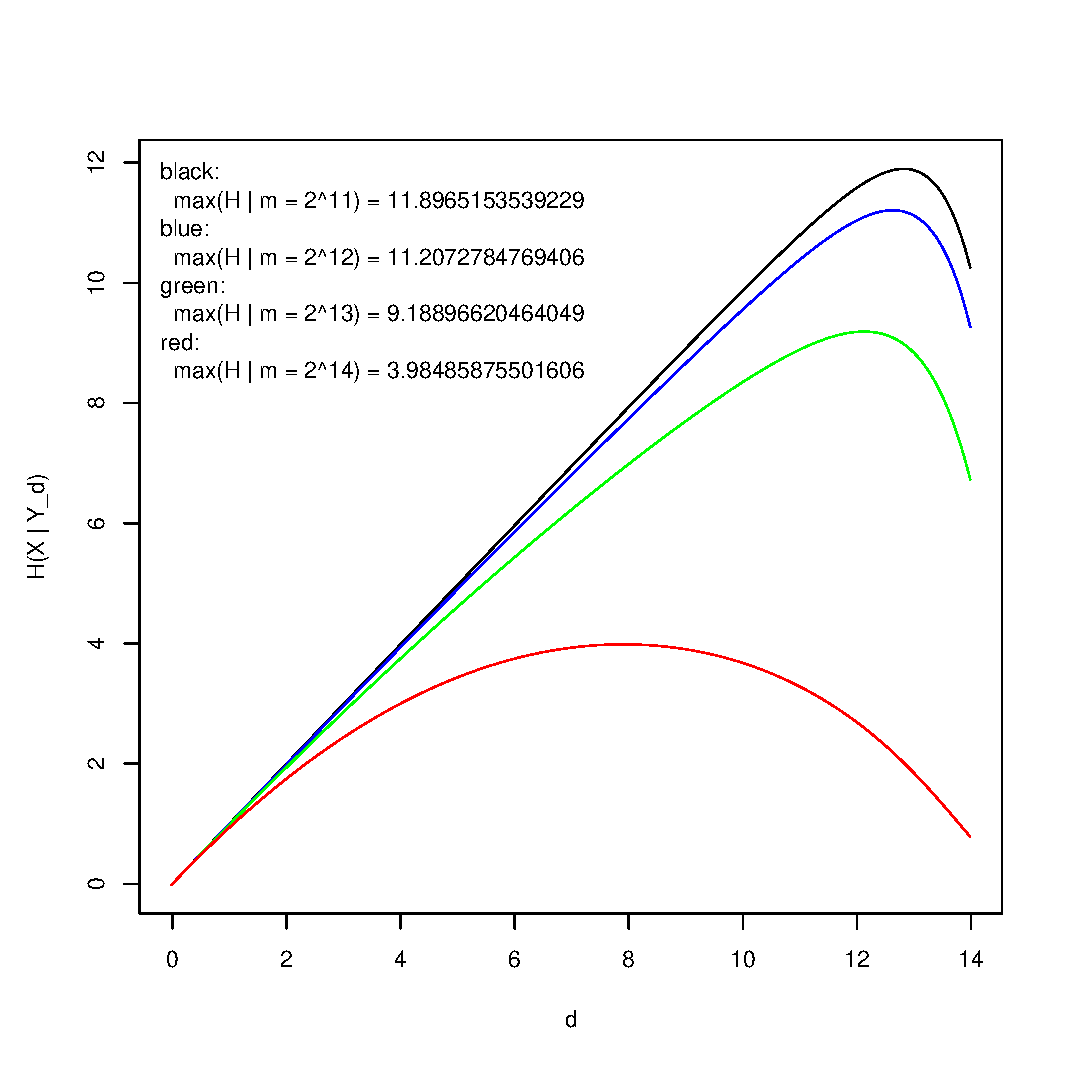
\includegraphics[width=3in, trim=0mm 0mm 0mm 20mm]{lb_m.eps}
		\caption{Lower Bound over d}\label{lb_m}
		\end{figure}		

		Since our lower bound in theorem \ref{thm1} is a maximum value
		over $d$, the $x$-axis is $d$ and the peak of each line
		is the lower bound for each $m$. As it shows, when $m = 2^{12} = 4096$, the lower
		bound is about $11.1$. 
		Thus only one update operation after thousands of index calculations is required
		to guarantee a lower bound higher than $10$.
		
		In fact, the proved lower bound in theorem \ref{thm1} is so
		simple and the tight lower bound is expected to be much higher
		for the following reasons.
		Observing the proof of theorem \ref{thm1}, only the
		entropy in the situation $Y = \alpha$ is count. However, in
		many situations that $Y = \beta$, there is still a high entropy.
		What's more, $B = false$ is also assumed so the attacker is
		given an extra information about whether all his enumerated $x$
		in recent $d$ updates are in candidate set $C_d$. But
		in real situation, this is unknown to the attacker.
		
	\subsection{Experimental Evaluation}
		For convenience, define
		\begin{align*}
		 p_1 &= p(B = false)\\
		 p_2 &= p(|C_d| = 2^d)\\
		 p_3 &= p(|K_i| = 0 \; (i \leq 0 < d) \; \backslash |C_d| = 2^d)
		\end{align*}
		In our proof above, $p_1$,
		$p_2$ and $p_3$ are 
		three key points to the final result.
		Lower bound for each of them has been proved
		and lower bound of $H(X | Y_d)$ is achieved by:
		\begin{align*}
			H(X | Y_d) &\geq p_1 \cdot p_2 \cdot p_3 \cdot d
				\geq B(D, m, d)
		\end{align*}
		
		In fact, $p_1 \cdot p_2 \cdot p_3$ can be measured in a real program which 
		simulates the same behaviour as defender mechanism.
		So the proof above can be evaluated by this experiment.
		Moreover, this experiment will show how tight our lower bound is
		when $H(X | Y_d = \beta)$ and $H(A | B = true)$ are ignored.
		
		The experiment program simply simulates the whole process of $d$ updates
		for $10000$ times and records the number of successful events
		to estimate the possibility $p_1 \cdot p_2 \cdot p_3$.
		
		Figure \ref{p13}, \ref{p14} show the result when $m = 2^{13}, 2^{14}$
		
		\begin{figure}[!t]
		\centering
		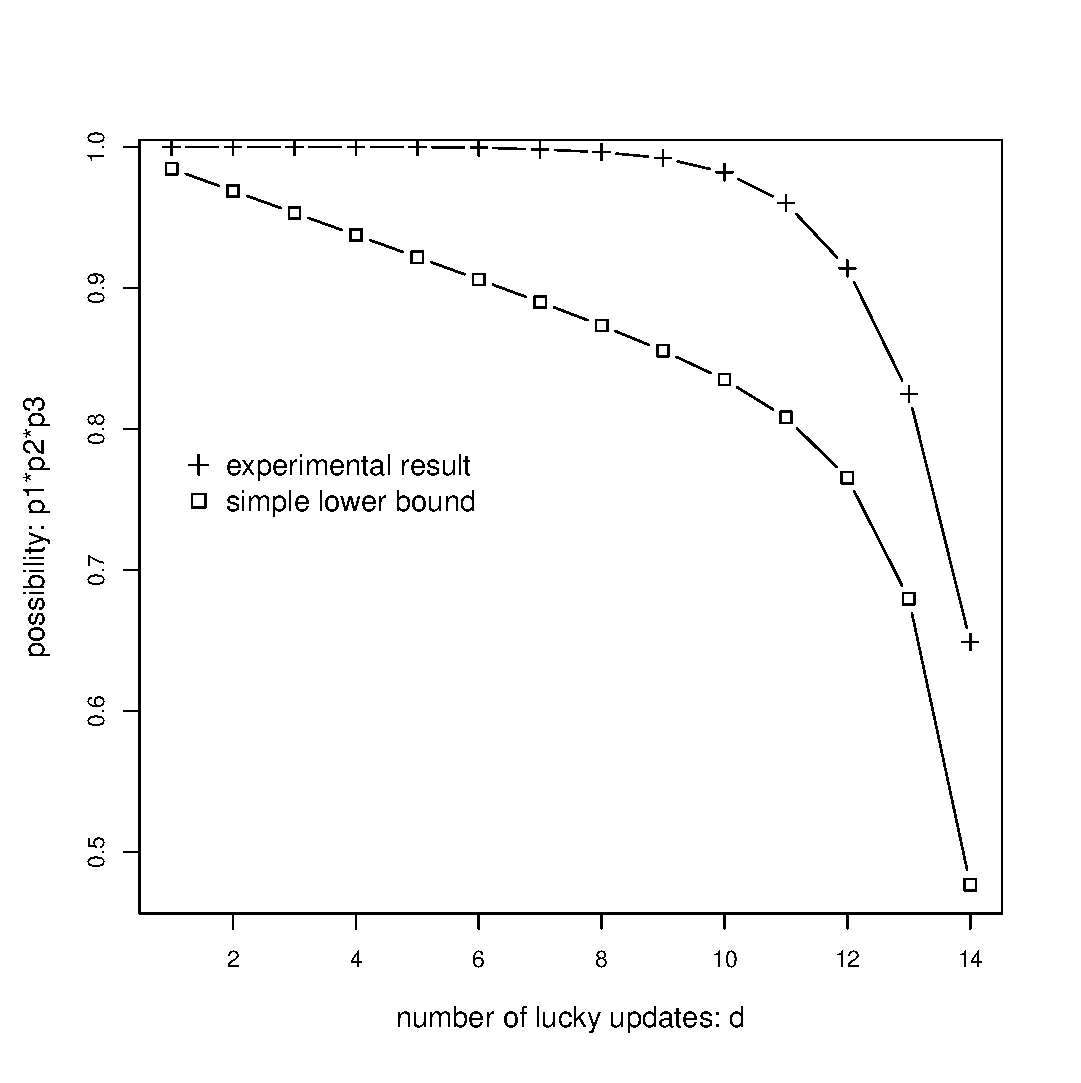
\includegraphics[width=3in, trim=0mm 0mm 0mm 20mm]{p13.eps}
		\caption{$p_1 \cdot p_2 \cdot p_3$ when $m = 2^{13}$}\label{p13}
		\end{figure}

		\begin{figure}[!t]
		\centering
		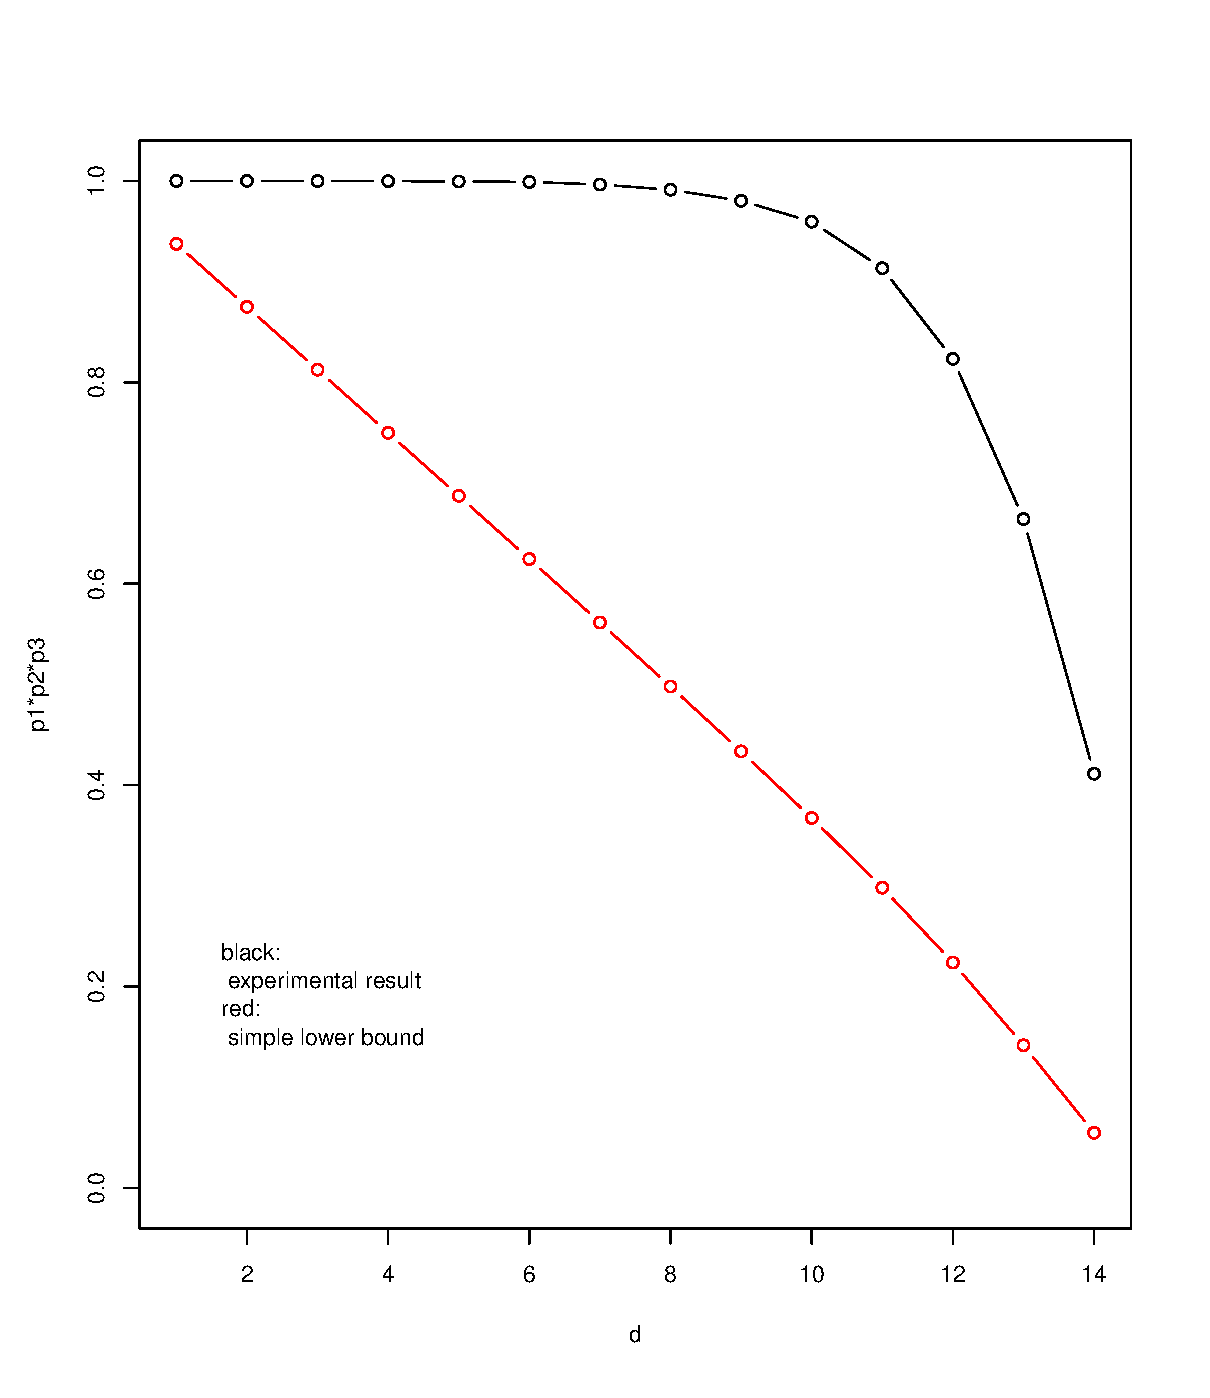
\includegraphics[width=3in, trim=0mm 0mm 0mm 20mm]{p14.eps}
		\caption{$p_1 \cdot p_2 \cdot p_3$ when $m = 2^{13}$}\label{p14}
		\end{figure}
		
		It can be seen that the simple lower bound is not too
		far away from the experimental result when $m = 2^{13}$.		
		However when $m = 2^{14}$, the simple lower bound
		estimated is much smaller than experimental result. Therefore,
		there is still plenty of room to improve the lower bound
		to make it tight, even if $H(X | Y_d = \beta)$ and $H(A | B = true)$ 
		are ignored. Meanwhile, the lower bound that can be proved should
		be higher than we simply get from theorem \ref{thm1}.
		For example, when $m = 14$, the experimental result
		of $p_1 \cdot p_2 \cdot p_3$ shows a lower bound of $10$
		when $d = 11$, while our simple lower bound only shows $4$
		when $d = 8$.
		
		To check that the simple lower bound is far from the experimental
		result only for large $m$, one more experiment is conducted
		for $m = 2^{11}$ and shown in figure \ref{p11}
		which confirms that our estimation
		of $p_1, p_2, p_3$ is correct and accurate for small $m$.

		\begin{figure}[!t]
		\centering
		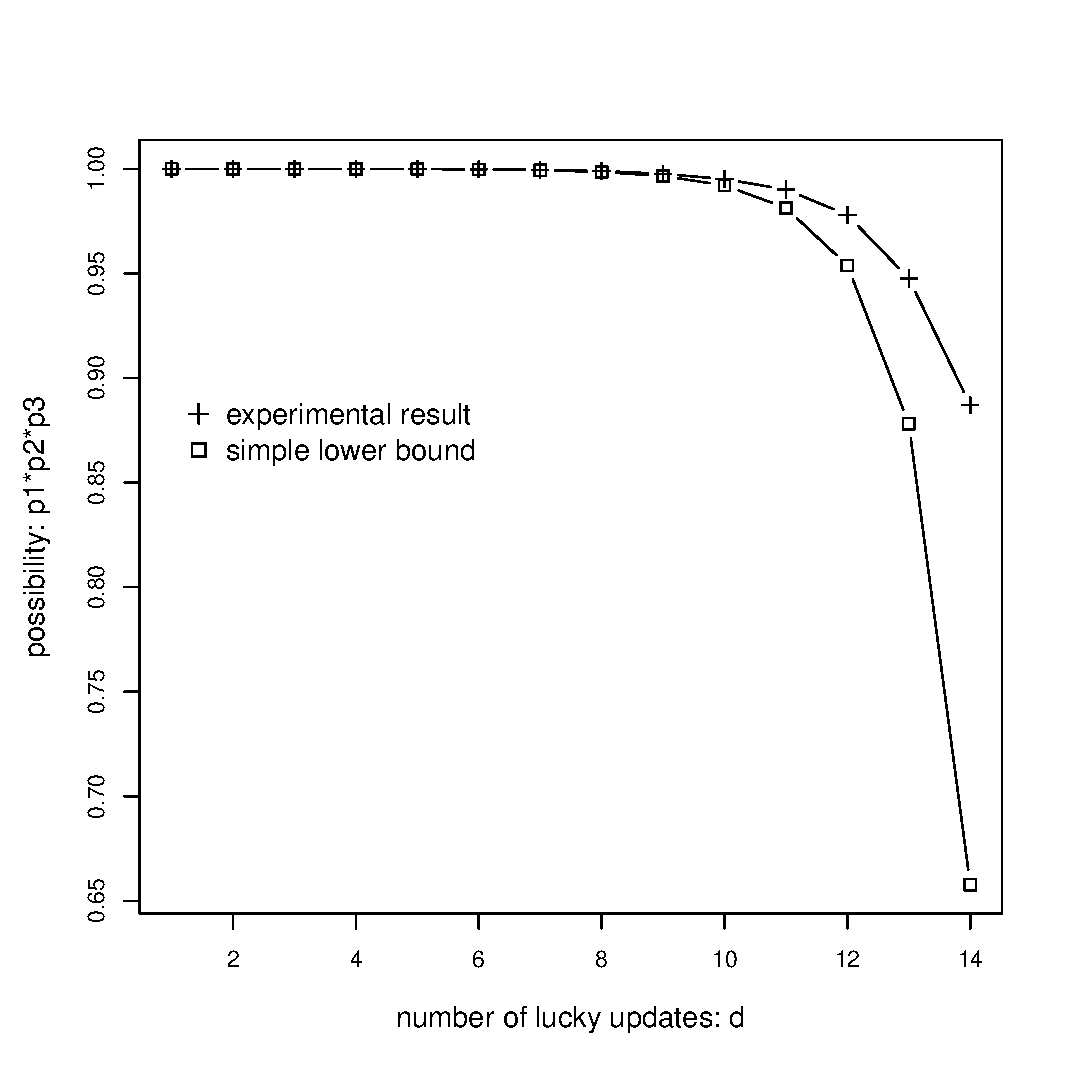
\includegraphics[width=3in, trim=0mm 0mm 0mm 20mm]{p11.eps}
		\caption{$p_1 \cdot p_2 \cdot p_3$ when $m = 2^{11}$}\label{p11}
		\end{figure}
		
		In sum, it has been evaluated that our simple lower bound
		is valid while it is not so tight even if we ignore
		$H(X | Y_d = \beta)$ and $H(A | B = true)$, especially
		when $m$ is large. In the experiment,
		it shows that when $D = 32$ and $m = 2^{14} = 16384$, the lower bound
		is still at least $10$.

\subsection{Essential Meaning based on Min-Entropy}
	All the analysis above is based on Shannon entropy.
	And min-entropy $H_\infty(X)$ define the entropy in a new way that
	\begin{align*}
		H_\infty(X) = \min_{x \in \mathcal X} \left(-\log p\left(X = x\right) \right)
	\end{align*}
	Similar conditional min-entropy could also be defined.
	
	The simple proof above also applies to this min-entropy
	because $p(x | Y = y)$ is either $0$ or $2^{-d}$ which implies:
	\begin{align*}
		-log(0) = \infty > -log(2^{-d}) = d
	\end{align*}
	And the lower bound for Shannon entropy and min-entropy 
	in our proof is the same for the same reason.
	As it can be seen that min-entropy's definition looks simpler, 
	it's easier to find out the meaning of the lower
	bound for conditional min-entropy. For min-entropy with a deterministic condition,
	$H_\infty(X | Y = y) = h$
	denotes the highest probability $2^{-h}$ that adversary can achieve to guess
	the right answer when $Y = y$ is known.
	Since $H_\infty(X | Y) = E\left(H_\infty(X | Y = y)\right)$,
	conditional min-entropy means the expected highest
	possibility that one adversary can guess the right answer.
	Therefore, the proof of our lower bound shows that
	the expected highest possibility that a computationally-unbounded
	adversary can guess the right plain text is very small: $2^{-\Omega(D)}$.
	And it's $2^{-10}$ in the special case for $D = 32$ and $m = 2^{12}$.
	
	Since $h$ is either $d$ or $0$ in our proof,
	$H_\infty(X | Y)$ is
	\begin{align*}
		E\left(H_\infty(X | Y = y)\right) &= p\left(H_\infty(X | Y = y) = d\right) \cdot d\\
		 &= p_1 \cdot p_2 \cdot p_3 \cdot d
	\end{align*}
	where $p_1 \cdot p_2 \cdot p_3$ is the chance to still confuse the adversary with 
	$2^d$ equally possible uncertainties.
	
	So as in the graph of $p_1 \cdot p_2 \cdot p_3$ when 
	$m = 2^{11}$ displayed above, both simple lower
	bound and experimental result show that
	there is a chance greater than $95\%$ percent that the adversary
	will be confused with $2^{12}$ equally possible uncertainties
	even if he or she is computationally-unbounded and has been attacking
	for an infinite long time, as long as one defend operation is enforced
	after $2^{11}$ index calculations.

% An example of a floating figure using the graphicx package.
% Note that \label must occur AFTER (or within) \caption.
% For figures, \caption should occur after the \includegraphics.
% Note that IEEEtran v1.7 and later has special internal code that
% is designed to preserve the operation of \label within \caption
% even when the captionsoff option is in effect. However, because
% of issues like this, it may be the safest practice to put all your
% \label just after \caption rather than within \caption{}.
%
% Reminder: the "draftcls" or "draftclsnofoot", not "draft", class
% option should be used if it is desired that the figures are to be
% displayed while in draft mode.
%
%\begin{figure}[!t]
%\centering
%\includegraphics[width=2.5in]{myfigure}
% where an .eps filename suffix will be assumed under latex, 
% and a .pdf suffix will be assumed for pdflatex; or what has been declared
% via \DeclareGraphicsExtensions.
%\caption{Simulation Results}
%\label{fig_sim}
%\end{figure}

% Note that IEEE typically puts floats only at the top, even when this
% results in a large percentage of a column being occupied by floats.


% An example of a double column floating figure using two subfigures.
% (The subfig.sty package must be loaded for this to work.)
% The subfigure \label commands are set within each subfloat command, the
% \label for the overall figure must come after \caption.
% \hfil must be used as a separator to get equal spacing.
% The subfigure.sty package works much the same way, except \subfigure is
% used instead of \subfloat.
%
%\begin{figure*}[!t]
%\centerline{\subfloat[Case I]\includegraphics[width=2.5in]{subfigcase1}%
%\label{fig_first_case}}
%\hfil
%\subfloat[Case II]{\includegraphics[width=2.5in]{subfigcase2}%
%\label{fig_second_case}}}
%\caption{Simulation results}
%\label{fig_sim}
%\end{figure*}
%
% Note that often IEEE papers with subfigures do not employ subfigure
% captions (using the optional argument to \subfloat), but instead will
% reference/describe all of them (a), (b), etc., within the main caption.


% An example of a floating table. Note that, for IEEE style tables, the 
% \caption command should come BEFORE the table. Table text will default to
% \footnotesize as IEEE normally uses this smaller font for tables.
% The \label must come after \caption as always.
%
%\begin{table}[!t]
%% increase table row spacing, adjust to taste
%\renewcommand{\arraystretch}{1.3}
% if using array.sty, it might be a good idea to tweak the value of
% \extrarowheight as needed to properly center the text within the cells
%\caption{An Example of a Table}
%\label{table_example}
%\centering
%% Some packages, such as MDW tools, offer better commands for making tables
%% than the plain LaTeX2e tabular which is used here.
%\begin{tabular}{|c||c|}
%\hline
%One & Two\\
%\hline
%Three & Four\\
%\hline
%\end{tabular}
%\end{table}


% Note that IEEE does not put floats in the very first column - or typically
% anywhere on the first page for that matter. Also, in-text middle ("here")
% positioning is not used. Most IEEE journals/conferences use top floats
% exclusively. Note that, LaTeX2e, unlike IEEE journals/conferences, places
% footnotes above bottom floats. This can be corrected via the \fnbelowfloat
% command of the stfloats package.



\section{Conclusion}
	To ensure the security of deterministic encryption
	for low entropy PII such as cellphone numbers,
	this paper briefly presents a novel defender model as well
	as a defender mechanism implemented for a specific
	OSN which uses cellphone numbers to generate encrypted indexes. 
	The defender mechanism also applies to PII other than
	cellphone numbers.
	
	This paper mainly focuses on analysis of this defender mechanism.
	A lower bound of conditional entropy is calculated to
	prove the mechanism's security for even
	computationally-unbounded adversaries.
	At the same time, the system's efficiency is also kept.
	Asymptotically, suppose that the original entropy is $D$,
	a lower bound for conditional entropy of $\Omega(D)$ can be
	guaranteed when only one defend operation is required after
	$2^{\Omega(D)}$ attacks.
	Based on min-entropy, our proof shows that
	such an adversary only has an expected chance 
	less than $2^{-\Omega(D)}$ to guess the right plain text.
	However, the lower bound derived
	is believed to be not so tight. 
	Conducted experiments confirm that the proved lower bound is valid while
	the tight lower bound
	should be much higher even if a lot of things are ignored.
	
	In short, it's theoretically secured and should be more practically secured.	
	
% conference papers do not normally have an appendix


% use section* for acknowledgement
%\section*{Acknowledgment}
%
%
%The authors would like to thank...
%more thanks here


% trigger a \newpage just before the given reference
% number - used to balance the columns on the last page
% adjust value as needed - may need to be readjusted if
% the document is modified later
%\IEEEtriggeratref{8}
% The "triggered" command can be changed if desired:
%\IEEEtriggercmd{\enlargethispage{-5in}}

% references section

% can use a bibliography generated by BibTeX as a .bbl file
% BibTeX documentation can be easily obtained at:
% http://www.ctan.org/tex-archive/biblio/bibtex/contrib/doc/
% The IEEEtran BibTeX style support page is at:
% http://www.michaelshell.org/tex/ieeetran/bibtex/
%\bibliographystyle{IEEEtran}
% argument is your BibTeX string definitions and bibliography database(s)
%\bibliography{IEEEabrv,../bib/paper}
%
% <OR> manually copy in the resultant .bbl file
% set second argument of \begin to the number of references
% (used to reserve space for the reference number labels box)

\bibliographystyle{IEEEtran}
\bibliography{IEEEabrv,paper}

%\begin{thebibliography}{1}
%
%\bibitem{cond_entropy:2}
%C. Arndt (2001). \emph{Information Measures: Information and its description in Science and Engineering)}. 
%\hskip 1em plus 0.5em minus 0.4em\relax Berlin: Springer. pp. 370C373. ISBN 3-540-41633-1.
%
%\end{thebibliography}

% that's all folks
\end{document}


